\chapter{Assignment 2: Basic Probabilities and Visualizations}

\section{Task a}
For the given samples (Variable X and Y) a scatter plot deems to be the most suitable candidate to plot the given points. This can be said because scatter plot helps to show the relationship between two variables, as one can see where the different points lie in the graph. This tells us how co-related the samples are.

\begin{figure}[h!]
\centering
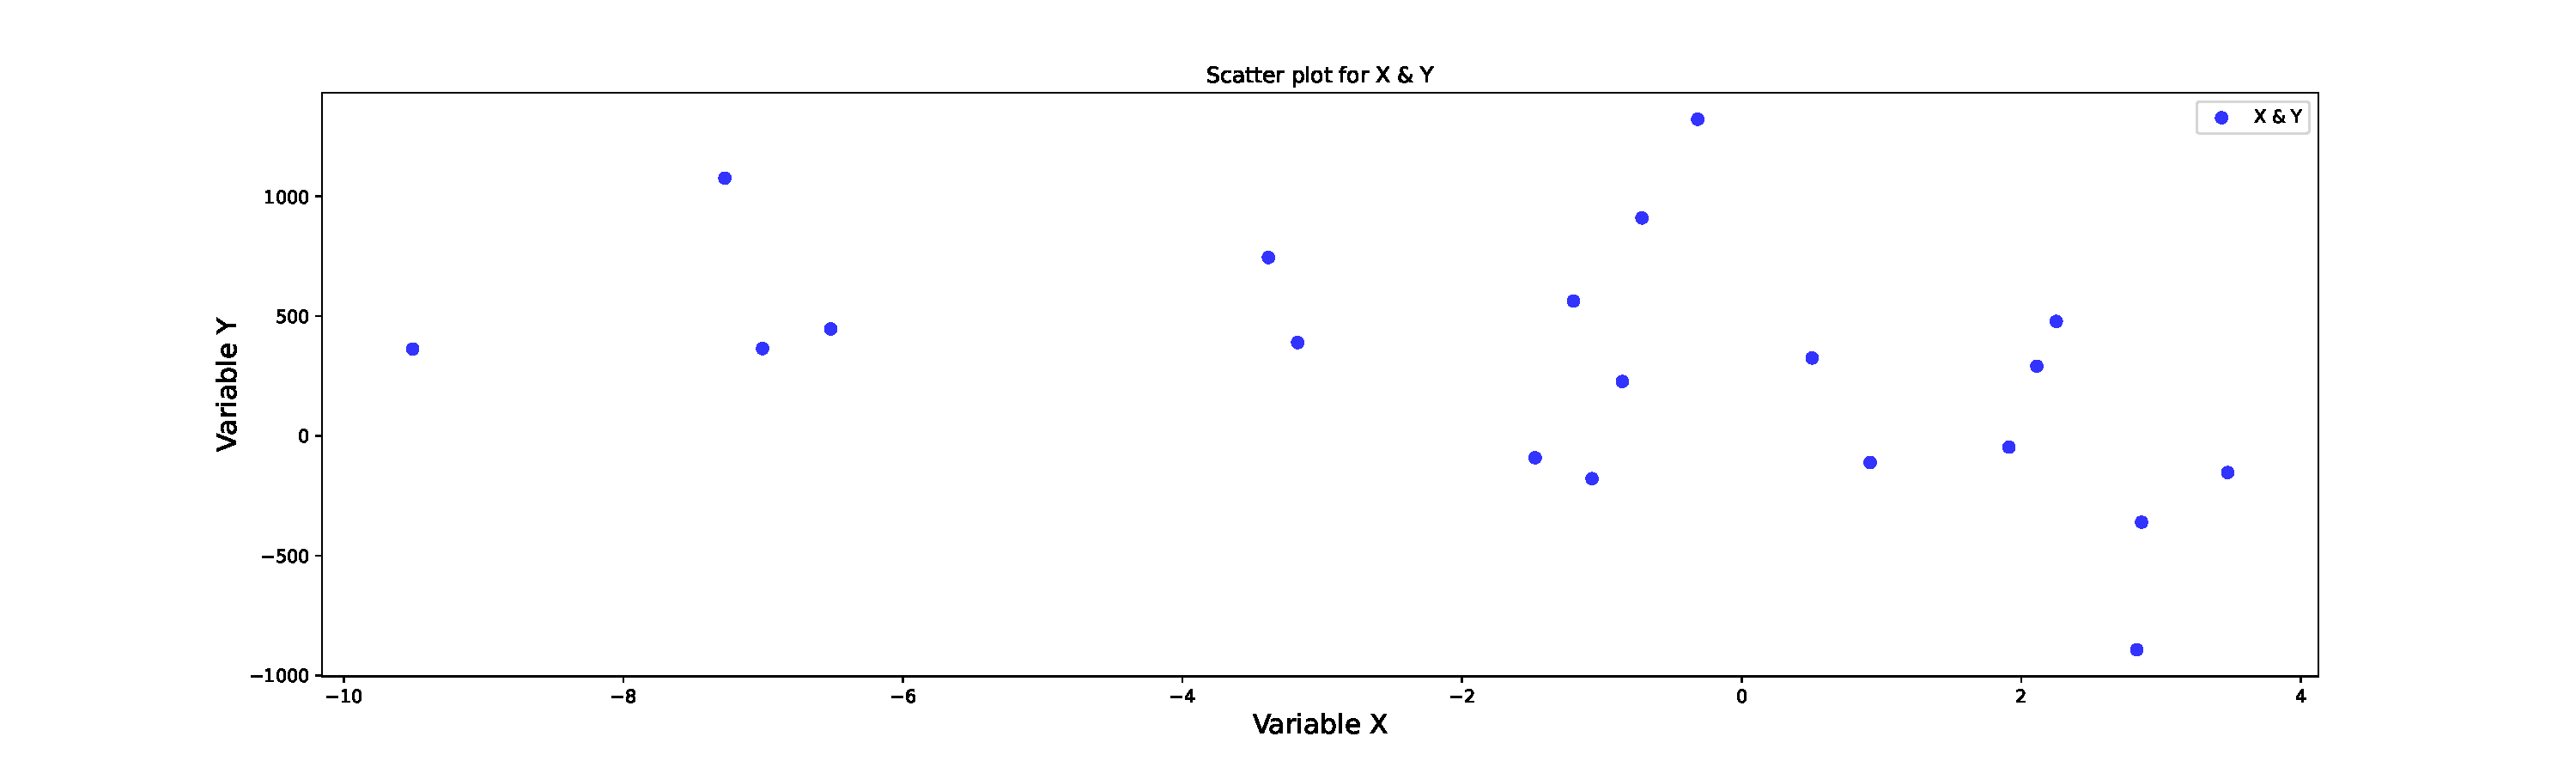
\includegraphics[width=\textwidth]{pics/task_2_a.pdf}
\caption{Scatter Plot for X and Y}\label{fig:task_2_a}
\end{figure}
\FloatBarrier
A simple look in the scatter plot in figure \ref{fig:task_2_a} shows us the data has a very large covariance as the points in the graph are very sparsely distributed in the plot.

\begin{lstlisting}[caption={Plotting the Scatter Plot with Variance Calculations)},label={lst:code_task_2_a}]
import numpy as np
import matplotlib.pyplot as plt

# Definitions
sample_data = [(2.919, 601.99), (5.057, -407.77), (1.168, -399.27), (6.401, 599.08), (0.973, 193.58), (-8.109, 1738.46),(2.883, 380.56), (3.652, -354.4), (-8.509, 591.96), (-8.886, -87.1), (-1.664, -1748.93),(-0.557, -57.74), (-15.28, 518.67), (-1.852, -56.12), (0.092, 434.48), (-6.536, -128.93),(-1.547, -696.37), (-1.281, -323.53), (6.454, -62.28), (-7.779, 614.93)]

# Plot the probability distribution
fig, ax = plt.subplots(1, 1, figsize=(20, 6))

# Separate value of X and Y from sample data
x, y = zip(*sample_data)

plt.scatter(x, y, color='b', label='X & Y', alpha=0.8)
plt.title('Scatter plot for X & Y')
plt.xlabel('Variable X', fontsize=15)
plt.ylabel('Variable Y', fontsize=15)

# Mean and covariance
mean_x = sum(x) / len(x)
mean_y = sum(y) / len(y)
x_minus_mean_x = np.asarray(x) - mean_x
y_minus_mean_y = np.asarray(y) - mean_y

# Covariance of X & Y
cov_x_y = sum(x_minus_mean_x * y_minus_mean_y) / len(x)
# Variance of X
var_x = sum(np.power(x_minus_mean_x, 2)) / len(x)

# Variance of Y
var_y = sum(np.power(y_minus_mean_y, 2)) / len(y)

plt.legend()
plt.savefig('images/task_2_a.pdf')
\end{lstlisting}

\subsubsection{Mean \& Covariance}   

The mean of Variables can be calculated using E[X]=  $\frac{1}{N} \sum_{i=1}^{N}x_i$  (\cite{Iubh:2021}) where N=20 is the total number of samples and the numerator is the sum of the random variable X or Y. Using this formula, the expectation ($\mu$) of the variable X and Y are calculated. E[X] = $\mu_x$= -1.62 and E[Y] = $\mu_y$= 67.56 \newline 
The Covariance of two variables can be calculated using cov(X,Y) =  $\frac{1}{N} \sum_{i=1}^{N}(x_i - \mu_x)^2 (y_i - \mu_y)$ (\cite{Iubh:2021}). Using the given formula the is cov(X,Y)= -1040.32.\newline
Similarly, the Variance can be calculated using var[X]=$\frac{1}{N} \sum_{i=1}^{N}(x_i - \mu_x)^2$. The calculated variances are as follows Var[X]=32.629 and Var[Y]= 4.578e+5.

\section{Task b}
It is given that a ball is thrown at a random angle $\theta \in$ [0, 360) which is in degrees and in a random radius r $\in$ [0, 1] which are both independent and uniform. Due to the fact the random variables are uniform we can easily define their respective density functions f($\theta$) = $\frac{1}{360}$ and f(r) = 1. This can be calculated because the PDF of a uniformly distributed function is given by 

\begin{equation}
    f(x) = \frac{1}{b-a}  x \in [a, b] \text{( \cite{openstax} , pg. 317)}
\end{equation} 
Since both of the random variables $\theta$ and r are independent we can also calculate the joint density function $f_{r,\theta}(r, \theta) = f(r) f(y) =  1 \times \frac{1}{360} = \frac{1}{360}$. We can see that the given random variables r and $\theta$ are the polar coordinates which lie within a unit circle. This can be said because the support of r is [0, 1] and has an angle $\theta$ (0, 360) degrees which would depict a circle.\newline 
Furthermore, with the polar coordinates, we can transform the variable f(r, $\theta$) $\rightarrow$ f(x,y) with $-1<x< 1$ and $-1 < y< 1$. Using simple trigonometry we can derive the simple relationship of the points x and y lying in the Cartesian coordinates which are x = r cos($\theta \times \frac{\pi}{180}$) and  y = r sin($\theta \times \frac{\pi}{180}$).It is to be noted that the angle given is in degrees and they must be converted to radians as our given angle is in degrees.\newline 
Therefore, solving for r and $\theta$ we get an inverse h = $g^{-1}(x,y)$
\begin{cases*}\label{eqn:task_2_c_inverse}
   r= $\sqrt{x^2+y^2}$&\text{= $h_1(x,y)$}
    &\\ $\theta = \frac{180}{\pi} \arctan(\frac{y}{x})$&\text{= $h_2(x,y)$}
\end{cases*}.\newline\newline
Now we can apply the transformation theorem (\cite{Iubh:2021}, pg.94) to get the density $f(x,y)$. The formula for the transformation is as follows:
\begin{equation} \label{eqn:transform_task_2_b}
    f(x,y) = f_{r,\theta}(x,y) \times \begin{vmatrix}
    J_{g^{-1}(x,y)}
    \end{vmatrix}
\end{equation}
The determinant of the Jacobian matrix $J_{g^{-1}(x,y)}$ is needed in order to continue forward to calculate the joint density function of x and y. The steps to calculate the Jacobian matrix are as follows:
\begin{enumerate}
    \item $\frac{\partial {h_1}}{\partial {x}} = \sqrt{x^2 +y^2} dx$
    \item $\frac{\partial {h_1}}{\partial {x}} = \frac{2x}{2\sqrt{x^2+y2}}$ Using the chain rule for parital derivative and substituting u=$\sqrt{x^2 +y^2}$ 
     \item $\frac{\partial {h_1}}{\partial {x}} = \frac{x}{\sqrt{x^2+y2}}$ 
     
     \item $\frac{\partial {h_1}}{\partial {y}} = \sqrt{x^2 +y^2} dy$
     \item $\frac{\partial {h_1}}{\partial {y}} = \frac{y}{\sqrt{x^2+y2}}$ Using the chain rule for parital derivative and substituting u=$\sqrt{x^2 +y^2}$ 
     
     \item $\frac{\partial {h_2}}{\partial {x}} = \frac{180}{\pi}arctan(\frac{y}{x}) dx$
     \item $\frac{\partial {h_2}}{\partial {x}} = \frac{180}{\pi}\frac{-y}{x^2+y^2}$ Using the chain rule for parital derivative and substituting u=$arctan(\frac{y}{x})$
     \item $\frac{\partial {h_2}}{\partial {y}} = \frac{180}{\pi}arctan(\frac{y}{x}) dy$
    \item $\frac{\partial {h_2}}{\partial {y}} = \frac{180}{\pi}\frac{x}{x^2+y^2}$ Using the chain rule for parital derivative and substituting u=$arctan(\frac{y}{x})$.
    
    \item $J_{g^{-1}(x,y)}$ = \begin{vmatrix}
    \frac{\partial {h_1}}{\partial x} & \frac{\partial {h_1}}{\partial y} \\
    \frac{\partial {h_2}}{\partial x} & \frac{\partial {h_2}}{\partial y}
    \end{vmatrix} Calculating the Jacobian matrix
    
    \item $J_{g^{-1}(x,y)}$ = \begin{vmatrix}
    \frac{2x}{2\sqrt{x^2+y2}} & \frac{y}{\sqrt{x^2+y2}} \\
    \frac{180}{\pi}\frac{-y}{x^2+y^2} & \frac{180}{\pi}\frac{x}{x^2+y^2}
    \end{vmatrix}
    
    \item $|J_{g^{-1}(x,y)}|$ = $\frac{180}{\pi} \frac{x^2}{\sqrt{x^2+y^2}(x^2+y^2)}+ \frac{180}{\pi}\frac{y^2}{\sqrt{x^2+y^2}(x^2+y^2)}$ Calculating the determinant $\frac{\partial {h_1}}{\partial x}\times \frac{\partial {h_2}}{\partial y} - \frac{\partial {h_1}}{\partial y} \times \frac{\partial {h_2}}{\partial x}$
    \item $|J_{g^{-1}(x,y)}|$ = $ \frac{180}{\pi}\frac{1}{\sqrt{x^2+y^2}}$
\end{enumerate}
Using the equation (see \ref{eqn:transform_task_2_b}) we can acquire the joint density function of f(x,y)= $\frac{1}{360}\frac{180}{\pi}\frac{1}{\sqrt{x^2+y^2}} = \frac{1}{2\pi}\frac{1}{\sqrt{x^2+y^2}}$ where the support of the transformed variable is $x^2+y^2 \leq 1$. This is because the value of X and Y are both bounded with the respect to the maximum possible radius 1.
\begin{equation}\label{eqn:density_task_2_b}
   f(x,y) =  \begin{cases*}
   \frac{1}{2\pi}\frac{1}{\sqrt{x^2+y^2}} &\text{ $x^2+y^2 \leq 1$}
    &0&\text{elsewhere}
\end{cases*}
\end{equation}
Using the joint density function we can calculate the marginal density function f(x) and f(y) which are given as follows $f(x) = \int_{-\sqrt{1-x^2}}^{\sqrt{1-x^2}} f(x,y) dy $ and $f(y) = \int_{-\sqrt{1-y^2}}^{\sqrt{1-y^2}} f(x,y) dx .$
Calculating the densities of X and Y using the joint density.
\begin{enumerate}\label{eqn:density_x_task_2_b_sol}
    \item $f(x) = \int_{-\sqrt{1-x^2}}^{\sqrt{1-x^2}} f(x,y) dy $
    \item $f(x) = \int_{-\sqrt{1-x^2}}^{\sqrt{1-x^2}}  \frac{1}{2\pi}\frac{1}{\sqrt{x^2+y^2}} dy$ Using Trigonometric substitution (\cite{wiki:trig} Tangent substitution)
    \item Substituting y = x tan(u) and $dy = x sec^2(u)du$ (using the quotient rule) we get $\sqrt{x^2+y^2}= \sqrt{x^2+x^2tan^2}= \sqrt{x^2(1+tan^2(u)} = \sqrt{x^2sec^2(u)} = x sec(u)$. \newline After substituting the values from above we get  $f(x) = \frac{1}{2\pi}\int_{-\sqrt{1-x^2}}^{\sqrt{1-x^2}} \frac{xsec^2(u)}{x sec(u)} du = \frac{1}{2\pi}\int_{-\sqrt{1-x^2}}^{\sqrt{1-x^2}} sec(u) du$.
    \item Multiplying the numerator and denominator by tan(u) and sec(u), we get $f(x) = \frac{1}{2\pi}\int_{-\sqrt{1-x^2}}^{\sqrt{1-x^2}} \frac{sec^2(u) + sec(u)tan(u)}{sec(u)+tan(u)}du = \frac{1}{2\pi}\int_{-\sqrt{1-x^2}}^{\sqrt{1-x^2}}\frac{1}{s} ds = log(s).$
    \item Substituting $s = tan(u) + sec(u)$ and $ds = (sec^2(u) +tan(u)sec(u)$, we get $f(x) = \frac{1}{2\pi}\int_{-\sqrt{1-x^2}}^{\sqrt{1-x^2}} log(tan(u) + sec(u)) du .$
    \item we can substitute back $u = \tan^{-1}(\frac{y}{x})$, we get $f(x) = \frac{1}{2\pi}[log(tan(\tan^{-1}(\frac{y}{x}) + sec(\tan^{-1}(\frac{y}{x}))]_{-\sqrt{1-x^2}}^{\sqrt{1-x^2}} = \frac{1}{2\pi}[log(\frac{y}{x} + \sqrt{\frac{y^2}{x^2}}+1)]_{-\sqrt{1-x^2}}^{\sqrt{1-x^2}} = \frac{1}{2\pi}[log(y + \sqrt{y^2+x^2}) -log(x))]_{-\sqrt{1-x^2}}^{\sqrt{1-x^2}}$
    \item $f(x) = \frac{1}{2\pi} (log(\sqrt{1-x^2}+1) - log(x) - log(1-\sqrt{1-x^2})+ log(x))= \frac{1}{2\pi} (log(\sqrt{1-x^2}+1)- log(1-\sqrt{1-x^2})) $
\end{enumerate} 
Therefore the marginal density $f(x) = \frac{1}{2\pi} (log(\sqrt{1-x^2}+1)- log(1-\sqrt{1-x^2}))$. The marginal density for Y can be calculated using similar process (see steps in \ref{eqn:density_x_task_2_b_sol}) and the calculated density is $f(y) =  \frac{1}{2\pi} (log(\sqrt{1-y^2}+1)- log(1-\sqrt{1-y^2}))$

\subsubsection{ Mean \& Variance }
The expectation for X and Y can be computed using equation \ref{eqn:tasn2_b_mean}. However since our circle is a unit circle we can say that the limits for both X and Y range from [-1, 1]. This is because the radius of the circle r $\in [0, 1]$ and $\theta \in (0, 360]$ which goes around the whole circle ranging from -1 and 1.
\begin{equation} \label{eqn:tasn2_b_mean}
    E[X] = \int_{-\infty}^{\infty}xf(x) dx
\end{equation}
The calculation for the expectation for X is as follows:
\begin{enumerate}
    \item $E[X] = \int_{-1}^{1}xf(x) dx$
    \item $E[X] = \int_{-1}^{1}x\frac{1}{2\pi} (log(\sqrt{1-x^2}+1)- log(1-\sqrt{1-x^2})) dx$
    \item $E[X] = \int_{-1}^{1}x\frac{1}{2\pi} (log(\sqrt{1-x^2}+1)- log(1-\sqrt{1-x^2})) dx$
    \item $E[X] = \frac{1}{2\pi} (\int_{-1}^{1}(x log(\sqrt{1-x^2}+1))- \int_{-1}^{1}(x log(1-\sqrt{1-x^2}))) dx$
    \item We can see that both the functions $(x log(\sqrt{1-x^2}+1))$ and $(x log(1-\sqrt{1-x^2})))$ are odd functions as they satisfy the condition $f(-x) = -f(x)$. Therefore the area for them is 0 and the expectation $E[X]=\mu_x = 0$
\end{enumerate}
As the density function of Y is similar to that of X we can say that the expectation $E[Y]=\mu_y = 0$. Figure \ref{fig:task_2_b_odd_function} shows us as well that the total area under the curve for these functions are 0 and we can simplify our calculations by looking at the graph.

\begin{figure}[h!]
\centering
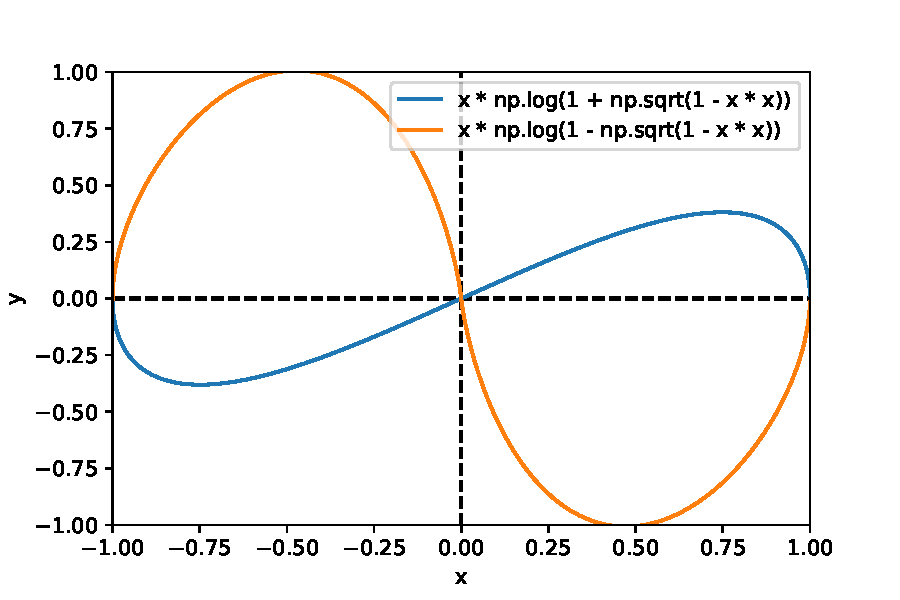
\includegraphics[width=\textwidth]{pics/task_2_b_odd_func.pdf}
\caption{Odd function for parts of the Expectation for functions X and Y}\label{fig:task_2_b_odd_function}
\end{figure}
\FloatBarrier

\begin{lstlisting}[caption={Code Task 2 b},label={lst:code_task_2_b}]
import numpy as np
import matplotlib.pyplot as plt

#Arrange
x=np.arange(-1, 1, 0.0001)
odd_first = x * np.log(1 + np.sqrt(1 - x * x))
odd_second = x * np.log(1 - np.sqrt(1 - x * x))
limits = [-1, 1]
plt.xlim(limits)
plt.ylim(limits)
# Set labels
plt.ylabel('y')
plt.xlabel('x')
axis= plt.gca()
# Plot
plt.plot(axis.get_xlim(), [0, 0], 'k--')
plt.plot([0,0], axis.get_ylim(),'k--')
plt.plot(x, odd_first, label= 'x * np.log(1 + np.sqrt(1 - x * x))')
plt.plot(x, odd_second, label='x * np.log(1 - np.sqrt(1 - x * x))')
plt.legend()
plt.savefig('images/task_2_b_odd_func.pdf')
\end{lstlisting}
\newpage The Variance can be calculated using the formula given below.
\begin{equation}
    Var[X]=\int_{-\infty}^{\infty}(x-\mu)^2f(x) dx
\end{equation}
The steps to calculate the variance for the random variable X is given below:
\begin{enumerate}
    \item $Var[X]=\int_{-1}^{1}(x-\mu_x)^2f(x) dx$ replacing the limits again with [-1,1].
    \item $Var[X]= \frac{1}{2\pi} \int_{-\infty}^{\infty}(x-0)^2  (log(\sqrt{1-x^2}+1)- log(1-\sqrt{1-x^2}))dx$ Since the expectation $E[X]$ is 0 we can substitute $\mu_x$ with 0.
    \item $Var[X]= \frac{1}{2\pi} \int_{-\infty}^{\infty}(x)^2  (log(\sqrt{1-x^2}+1)- log(1-\sqrt{1-x^2}))dx$
    \item $Var[X]= \frac{1}{2\pi} \int_{-\infty}^{\infty}x^2  (log(\sqrt{1-x^2}+1)- log(1-\sqrt{1-x^2}))dx$
    \item $Var[X]= \frac{1}{2\pi} \int_{-1}^{1}x^2log(\sqrt{1-x^2}+1)- \int_{-1}^{1} x^2log(1-\sqrt{1-x^2})dx$
    %\item $Var[X]= \frac{1}{2\pi} \int_{-\infty}^{\infty}- %\int_{-\infty}^{\infty} x^2log(1-\sqrt{1-x^2})dx .$ Using Integrating %by parts where $u_1= log(\sqrt{1-x^2}+1), v_1= x^2$ and $u_2 = %log(1-\sqrt{1-x^2}) and v_2=x^2$
    \item $Var[X]=\frac{1}{2\pi}(\frac{\pi}{6}-\frac{2}{9}+\frac{\pi}{6}-\frac{2}{9})$ As calculated by wolfram alpha (\cite{wolfram}), line 5 is the query used in wolfram to calculate the variance.
     \item $Var[X]=0.167$
\end{enumerate}
The Variance of Y is also similar because it has the same limits and similar density function. Therefore $Var[X] = 0.167$ and $Var[Y] = 0.167$